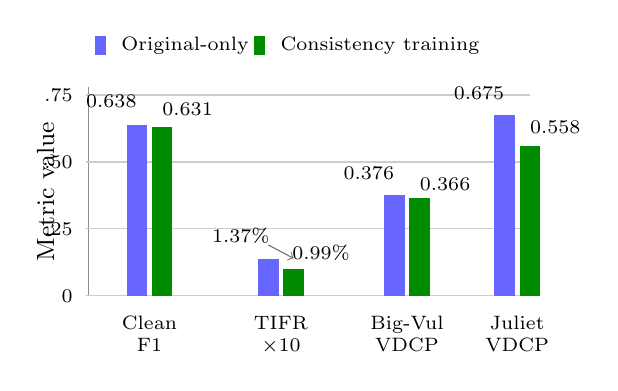
\begin{tikzpicture}[
  x=1.0cm,
  y=3.4cm,
  font=\small
]
\begin{scope}[shift={(0,-0.10)}]
\draw[black!45] (0,0) -- (5.6,0);
\draw[black!45] (0,0) -- (0,0.78);
\foreach \y/\label in {0/0,0.25/.25,0.50/.50,0.75/.75} {
  \draw[black!20] (-0.04,\y) -- (5.6,\y);
  \node[anchor=east, font=\scriptsize] at (-0.08,\y) {\label};
}
\node[anchor=center, rotate=90] at (-0.55,0.39) {Metric value};

% Clean F1
\fill[blue!60] (0.48,0) rectangle (0.74,0.638);
\fill[green!55!black] (0.80,0) rectangle (1.06,0.631);
\node[anchor=north, align=center, font=\scriptsize] at (0.77,-0.04) {Clean\\F1};
\node[anchor=south east, font=\scriptsize] at (0.73,0.666) {0.638};
\node[anchor=south west, font=\scriptsize] at (0.81,0.636) {0.631};

% TIFR scaled x10
\fill[blue!60] (2.15,0) rectangle (2.41,0.137);
\fill[green!55!black] (2.47,0) rectangle (2.73,0.099);
\node[anchor=north, align=center, font=\scriptsize] at (2.44,-0.04) {TIFR\\$\times 10$};
\node[anchor=south east, font=\scriptsize] at (2.42,0.157) {1.37\%};
\node[anchor=south west, font=\scriptsize] at (2.46,0.097) {0.99\%};
\draw[->, black!55] (2.28,0.19) -- (2.60,0.14);

% Big-Vul VDCP
\fill[blue!60] (3.75,0) rectangle (4.01,0.376);
\fill[green!55!black] (4.07,0) rectangle (4.33,0.366);
\node[anchor=north, align=center, font=\scriptsize] at (4.04,-0.04) {Big-Vul\\VDCP};
\node[anchor=south east, font=\scriptsize] at (4.00,0.398) {0.376};
\node[anchor=south west, font=\scriptsize] at (4.08,0.358) {0.366};

% Juliet VDCP
\fill[blue!60] (5.15,0) rectangle (5.41,0.675);
\fill[green!55!black] (5.47,0) rectangle (5.73,0.558);
\node[anchor=north, align=center, font=\scriptsize] at (5.44,-0.04) {Juliet\\VDCP};
\node[anchor=south east, font=\scriptsize] at (5.40,0.695) {0.675};
\node[anchor=south west, font=\scriptsize] at (5.48,0.568) {0.558};
\end{scope}

\fill[blue!60] (0.08,0.80) rectangle (0.22,0.87);
\node[anchor=west, font=\scriptsize] at (0.29,0.835) {Original-only};
\fill[green!55!black] (2.10,0.80) rectangle (2.24,0.87);
\node[anchor=west, font=\scriptsize] at (2.31,0.835) {Consistency training};
\end{tikzpicture}
